\documentclass[titlepage]{article}
\usepackage[]{algorithmic}
\usepackage[]{algorithm}
\usepackage[utf8]{inputenc}
\usepackage{listings}
\usepackage{amsmath}
\usepackage{qtree}
\qtreecenterfalse
\usepackage{nth}
\usepackage{caption}
\usepackage{tabulary}
\usepackage{subcaption}
\usepackage{fancybox}
\usepackage{graphicx}
\usepackage[letterpaper, portrait, margin=1in]{geometry}

\setlength{\parindent}{.5in}
\title{An empirical study of semantic similarity in WordNet and Word2Vec\vspace{5mm}}
\author{Abe Handler}
\date{\today}


\begin{document}
\thispagestyle{empty}
\begin{titlepage}
    \begin{center}
        \vspace{1in}
        
        \LARGE
        \textbf{An empirical study of semantic similarity in WordNet and Word2Vec}
        
        \vspace{3cm}
        A Thesis
        \vspace{3cm}
        
        Submitted to the Graduate Faculty of the 
        University of New Orleans 
        in partial fulfillment of the 
        requirements for the degree of 
        
        
        \vspace{2cm}
        
        Master of Science \\ in \\ Computer Science 
       
        \vspace{2cm}
        
        \vfill
        
        by \\
        \vspace{1cm}
        Abram Handler \\ 
        \vspace{1cm} 
        B.A. Columbia University, 2007 (Hons.) \\
        \vspace{1cm}
        December 2014
    \end{center}
\end{titlepage}

\pagenumbering{roman}
\setcounter{page}{2}
\tableofcontents

\Large
\begin{abstract}
This thesis performs an empirical analysis of Word2Vec by comparing its output to WordNet, a well-known, human-curated lexical database. It finds that Word2Vec tends to uncover more of certain types of semantic relations than others -- with Word2Vec returning more hypernyms than synonyms followed by meronyms, hyponyms and holonyms. Moreover, it shows the probability that neighbors separated by distance k in Word2Vec are semantically related in WordNet. This result both adds to our understanding of the still-unknown Word2Vec and helps to benchmark new semantic tools built from word vectors. 
\end{abstract}


\renewcommand{\thepage}{\arabic{page}}
\section{Introduction}

Word2Vec is a new unsupervised system for determining the semantic distance between words. For instance, after learning from billions of web pages, Word2Vec reports that the words \textit{Chinese river} are semantically close to the word \textit{Yangtze}. \cite{Word2VecWebsite} Such results have attracted lots of recent attention: over 100 researchers have cited Word2Vec since its publication in 2013. Yet certain aspects of the system's output are poorly understood. In particular: 

\begin{enumerate}
\item Word2Vec does not label particular semantic relationships between words -- like the synonomy between \textit{cold} and \textit{chilly} or the meronomy between \textit{wheel} and \textit{car}. Instead, it assigns a number between 0 and 1, indicating the semantic distance between two words\footnote{For instance, a Word2Vec model trained on the Google news corpus returns a semantic distance of .390 between \textit{truck} and \textit{tire} and a semantic distance of .168 between \textit{truck} and \textit{chicken}}. However, as Word2Vec’s creators note ``there can be many different types of similarities.” \cite{mikolov2013efficient} This opens a question: what sorts of semantic similarities does Word2Vec uncover?

\item Word2Vec can generate ranked lists showing which words are closer and which words are further way in a semantic model. For example, Word2Vec says that \textit{grandmaster} is \nth{3} from the word \textit{chess}, while \textit{Muay Thai kickboxing} is \nth{997}. \footnote{Word2Vec model trained on Google news corpus} What is the probability that two words that are k-apart in Word2Vec stand in some formal specific semantic relationship?
\end{enumerate}

This study seeks to answer such questions by comparing Word2Vec's output with WordNet -- a large, human-curated ``lexical database" \cite{Wordnetwebsite} which is the most-frequently cited ``lexiographic resource" \cite{widdows} in English. 

Such effort has several motivations. First, the study simply gives clearer knowledge of Word2Vec, which is still not well understood. Second, as researchers and practitioners build semantic tools from Word2Vec, they will inevitably turn to WordNet to evaluate their applications. Rei et. all \cite{rei2014looking} have already tried using WordNet to benchmark their Word2Vec-based hyponym detector. Accurately benchmarking such tools requires a clear understanding of the relationship between the two semantic systems. For instance, to evaluate Rei's study we must ask: what is the probability that Word2Vec will return a holonym from a random word at a semantic distance of k? This study establishes such a baseline for further research. 

\section{Related Work}

\subsection{Geometry and Meaning} \label{geom}
Computers are much better than humans at certain tasks, such as searching large lists or solving complex equations. However, Computer Science still struggles with the highly nuanced, contextually-dependent work of understanding a word's meaning. While automatic translation services might approximate some of our human intuitions about the meaning of a word or phrase, replicating all of the intricacy of natural language semantics remains an unsolved problem in computer science.

Efforts thus far have presumed a so-called distributional theory of semantics, which hypothesizes that those words which are distributed the same way in text or speech will have similar meanings. 

According to the distributional theory, the words \textit{keyboard} and \textit{piano} might occur together frequently in text because they refer to related things in the world. As the linguist JR Firth famously put it: ``a word is characterized by the company it keeps." \cite{firth} \footnote{Understanding natural language programmatically slides into philosophy and linguistics, where theorists and  have debated how words gain their meanings for millenia \cite{stanfordphilo}. We do not dig into the details of such debates here -- but instead take the distributional theory as given.}

Translating this linguistic insight into algorithmic formality often proceeds as follows: use all of the words and all of the documents in a corpus of text to form the rows and the columns of a large matrix. Project words or phrases into this semantic space. Words that have similar meanings are closer together. Words that have less similar meanings are farther apart.

As Dominic Widdows points out -- such algorithms form an unlikely connection between geometry (the mathematical study of space and objects in space) and semantics (the way a word refers to an object in the world). In other words: an unexpected link between geometry and meaning. \textit{Geometry and Meaning} \cite{widdows}. 

\subsection{Word2Vec}

Word2Vec follows very much in the geometric tradition detailed in section \ref{geom}. The algorithm uses complex, multi-level neural networks to project words into a semantic space, which can then be used to determine semantic distance or semantic proximity. The network is trained by giving positive feedback when words appear together in context and giving negative feedback when words are randomly swapped into other contexts. The output is a space filled with vector representations of words. Word vectors that are semantically closer together are more closely related than word vectors that are farther apart. 

This approach has garnered lots of attention and enthusiasm. Researchers have tried using Word2Vec to find the meaning of a word in context \cite{wang2014introduction}, to automatically determine human attitudes in text \cite{xue2014study} and even to ascertain political ideology \cite{iyyerpolitical}. 
Yet no empirical studies have yet attempted to systematically analyze output from Word2Vec in terms of the classical tool, WordNet. 

The gap is notable, in part, because researchers have begun to evaluate new semantic tools built on top of Word2Vec by using the human-curated WordNet, which remains the most-precise method for determining semantic relationships with a computer.

Rei et. all's ``Looking for Hyponyms in Vector Space" serves as an important example. \cite{rei2014looking} The researchers first use Word2Vec to find words with a particular semantic relationship (hyponomy) -- then look to WordNet to evaluate their method. Yet they presuppose certain relationships between WordNet and Word2Vec without providing any empirical justification -- writing that ``the most likely candidates for a high cosine similarity are synonyms, antonyms, hypernyms and homonyms". In section \ref{binary} we show that this is not the case. Word2Vec does not in fact return these semantic relations equally. 

Clearer understanding of how WordNet and Word2Vec are related will yield much precise evaluations. After all, both the linguistic mechanisms and the exact output of the Word2Vec system are still a bit mysterious. One popular explanation of the system concludes: ``Why does this produce good word representations? Good question. We don’t really know." \cite{goldberg2014word2vec}

\subsection{WordNet}  \label{WordNet}
WordNet has been a part of natural language processing for decades -- beginning at Princeton University in 1986. The system has its own logic and jargon, all built around the fundamental building block \cite{wordnet} of the ``synonymous set" (or synset) -- an unordered collection of ``cognitively synonymous words and phrases." \cite{cruse} Synsets are linked by relations, with particular relations linking particular words with particular parts of speech.

Thus, where Word2Vec represents words as vectors, WordNet models language with a large graph -- with semantically similar words (caled ``synsets") serving as the nodes and semantic relationships (such as the meronomy between \textit{tire} and \textit{car}) serving as the edges. \footnote{Because ``the majority of the WordNet’s relations connect words from the same part of speech (POS) ... WordNet really consists of four sub-nets, one each for nouns, verbs, adjectives and adverbs, with few cross-POS pointers."\cite{Wordnetwebsite}}

Five specific WordNet relationships concern us here:

\begin{itemize}

  \item \textbf{Synonomy}. WordNet can identify synonyms, words with the same meaning. For instance: \textit{roof} and \textit{ceiling}.
  \item \textbf{Hypernomy}. A word that is more general than some other word is said to be its hypernym. \textit{Language} is a hypernym of \textit{French}
  \item \textbf{Hyponomy}. A word that is more specific than some other word is said to be its hyponym. \textit{French} is a hyponym of \textit{language}
  \item \textbf{Meronomy}. A word that is a part of some other word is called a meronym. \textit{Bedroom} is a meronym of \textit{house}.
  \item \textbf{Holonomy}. If B contains A, B is a holonym of A. \textit{Japan} is a holonym of \textit{Fuji} because Fuji is in Japan.
\end{itemize}

Note that these are relationships between synsets, not between words. A word is associated with one or more synsets. A synset has a semantic relationship with other synsets. We explain our exact definition of semantic relation in the section \ref{method}.

\section{Method} \label{method}
If word vectors represent semantic similarity, we might expect a that two words that are a certain distance apart in Word2Vec have some semantic relationship in WordNet. We investigate with the following experiment. 

We begin with Google's word model, trained on 100 billion words in the Google news corpus \cite{Word2VecWebsite}. Then we select the set of 41600 unique words from the Reuters news corpus and, for each, we search for the closet 200 neighbors in the Word2Vec model. We then search WordNet for any semantic relationship between the original word and its neighbor -- concerning ourselves on with the semantic relations listed in section \ref{WordNet}.

For instance, our experiment might extract the word \textit{introduction} from the Reuters corpus and extract its 200 closest neighbors in Word2Vec. It might then find that k-th neighbor in Word2Vec is the word \textit{initiation}. It would then look up synsets for each word in WordNet see if the two words have any synsets in common. In this case, it would determine that the two words are synonyms because their synsets overlap with the synset 'initiation.n.01' -- defined as 'a formal entry into an organization or position or office'.

Note that this means that we use a binary measure to determine semantic relatedness in WordNet: if there is any overlap between the relevant synsets, we count the relation. If there is zero overlap between the synsets, we do not count the relation. Potential problems with such a binary measure are considered in section \ref{Jaccard}.

The process is very similar for other relations but the details warrant mention. Words can have multiple associated synsets in WordNet. When we search for holonyms, meronyms, hyponyms and hypernyms, we use a very wide measure of relatedness. For each synset associated with a word: we create a union of all associated relations from all synsets. If any synset from this union intersects with the synsets of the original word, we count the relation. Again, potential problems with such a measure are considered in section \ref{Jaccard}.

WordNet synsets are associated with a part of speech, but we do not consider them here. We discuss this further in section \ref{Future Work}.

\begin{algorithm}
\caption{Calculate the cosine distances associated with different semantic relations}
\begin{algorithmic}
\label{alg1}
\STATE $W \leftarrow words$
\FOR{$i=0$ to $len(W)$}
\STATE $N \leftarrow word2vec-neighbors(200)$
\FOR{$j=0$ to $len(W)$}
\IF{W[i] in wordnet} 

\IF{some condition is true}
\STATE record same stem and relation 
\ELSE
\IF{synononms(W[i], N[j])} 
\STATE record cosine distance and relation 
\ENDIF
\IF{meronyms(W[i], N[j])} 
\STATE record cosine distance and relation 
\ENDIF
\IF{hypernyms(W[i], N[j])} 
\STATE record cosine distance and relation 
\ENDIF
\IF{hyponyms(W[i], N[j])} 
\STATE record cosine distance and relation 
\ENDIF
\IF{holonyms(W[i], N[j])} 
\STATE record cosine distance and relation 
\ENDIF
\ENDIF

\ELSE
\STATE record not in WordNet

\ENDIF

\ENDFOR
\ENDFOR
\end{algorithmic}
\end{algorithm}

\subsection{Implementation Details}

There are a few important details surrounding the implementation of our experiment. 

\begin{enumerate}
  \item We allow two words to stand in multiple semantic relationships. For instance, a word is permitted to be both a hyponym and a holonym, if so labeled in WordNet. 
  \item We also keep track of words that do not appear in WordNet and words that have the same stem -- like \textit{nearing} and \textit{nears}. In these two cases, we do not search for the semantic relationships in WordNet because the relationship is already known.
  \item  We do not consider antonyms as Wordnet defines antonyms between words (not between synsets). All other relations are defined between synset, so antonyms are not an equal comparison. 
  \item  We access WordNet 3.0 and the Reuters-21578 \cite{rose2002reuters} corpus with the Python linguistics toolkit, NLTK \cite{BirdKleinLoper09}.
 \item  We access WordNet 3.0 and the Reuters-21578 \cite{rose2002reuters} corpus with the Python linguistics toolkit, NLTK 
 \item We access the Google news model via the popular python wrapper, Gensim \cite{gensim}.
 \item We use NLTK's snowball stemming tool to find words with the same stem. 
\end{enumerate}

\subsection{Processing results}

The experiment detailed in section \ref{method} lists the cosine distance between words. The section \ref{results} unpacks its findings. However, translating the output from the section \ref{method} into the results in \ref{results} requires an intermediate step: discovering how many of each relation maybe found within a given semantic distance. We do so by dividing 1 into 1000 equal parts using the numpy linspace method. Then, we loop through each of these parts -- and, for each, count how many of each type of relation are discovered beneath the threshold. The process is analogous to casting a wider and wider circle -- pulling in more and more relations as the circle expands.

\subsection{Adjusted counts}

Finally, some relations in WordNet have more associated synsets than others. Thus our experiment might be said to measure differences in associated synsets in WordNet instead of output from Word2Vec. We address this deficiency by generating adjusted counts that show the probability of each relation -- if all relations contained equally many synsets. We do this as follows. First we randomly sample 10,000 words from the Reuters corpus and determine the average number of associated synonyms, meronyms, holoynms, hypernyms and hyponyms. Then we average these averages to get an overall average number of associated synsets. To generate an adjusted count for some relation, we multiply the raw count by the overall average divided by the average for synset. Thus, if some synset has twice as many associated words than average its count will be halved. If some synset has half as many as the overall average, its count will be doubled.

\section{Results} \label{results}

\subsection{Raw numbers: A high-level overview} \label{raw}

Our first result is very clear: we show what sorts of relations are returned by Word2Vec. 

\begin{table}[ht]
\centering
\begin{tabular}{|l|l|}
\hline
Relation & Count \\  \hline
Holonym &  1453 \\  \hline
Meronym &  2561 \\  \hline
Hyponym &  25620 \\  \hline
Synonym &  37107 \\  \hline
Hypernym & 42908 \\  \hline
\end{tabular}
\captionsetup{justification=centering,margin=2cm}
\caption{Word2Vec captures far more of certain relations than others: \\ favoring synonyms, hyponyms and hypernyms ahead of holonyms and meronyms across the Reuters corpus}
\label{tab:my_label}
\end{table}

We find that Word2Vec favors synonyms and hypernyms and hyponyms ahead of meronyms and holonyms by an order of magnitude. These large differences across the entire corpus seem to indicate that Word2Vec picks up certain relationships ahead of others.

\begin{center}
\centering
\begin{figure}[!htbp]
  \centering
  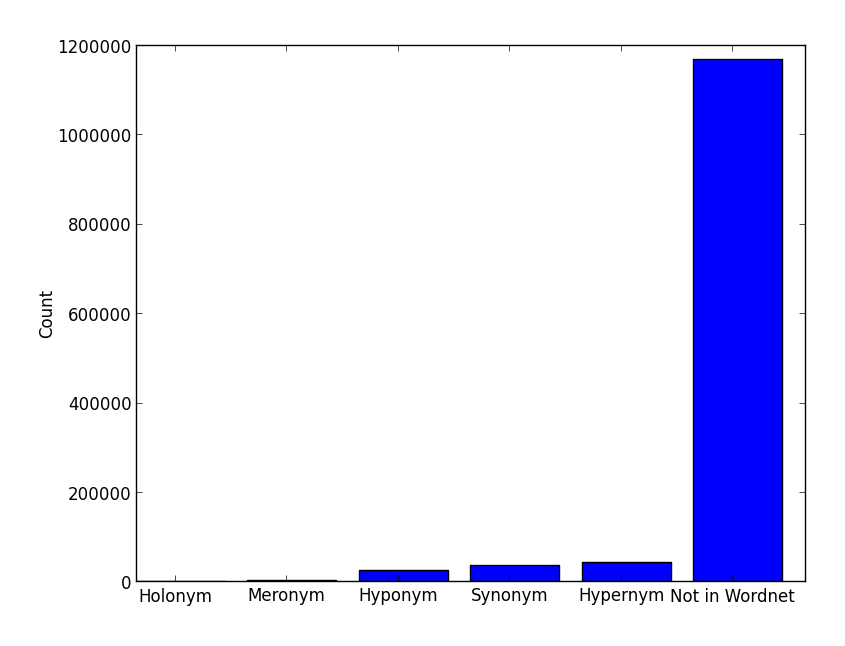
\includegraphics[scale=.5]{grand_total.png}
  \caption{Word2Vec more synonyms, hyponyms and hypernyms \\ than holonyms and meronyms}
  \label{fig:grand_total}
\end{figure}
\end{center}

We find that by far the largest category are those results that do not appear at all in WordNet. From our experiment, we find 1167354 such words from Word2Vec -- far too many to show in the chart above. This is because the model trained on the Google news corpus with Word2Vec is much, much larger than all of WordNet. Where WordNet 3 contains around 118,000 synsets \cite{wordnet}, the Word2Vec model in this experiments was trained on 100 billion words \cite{Word2VecWebsite} of news text. Most of the semantically similar words cannot be looked up in WordNet. For instance, \textit{Rohto Pharmaceutical} is not in WordNet: it's a big corporation, but not a household name in the United States. Thus WordNet has no way of determining its semantic relationship to the word \textit{industries}.\footnote{The Google news Word2Vec model lists the semantic distance between \textit{Rohto Pharmaceutical} and \textit{industries} at .494} It is not known how well the WordNet relations represent the mass of `semantically similar' words in Word2Vec. We consider this in section \ref{Future Work}.

\subsection{Counts by cosine distance} \label{cosine}

Cosine distance is a measure of the distance between the angle of two vectors. We analyzed the relative counts of different relations at different cosine distances and found that relations were not distributed uniformly. Hypernyms where distributed like hyponyms and synonyms. Holonyms were distributed like meronyms. Words with the same stem were distributed with a rough Gaussian curve.  

\begin{figure}[!htbp]
\centering
  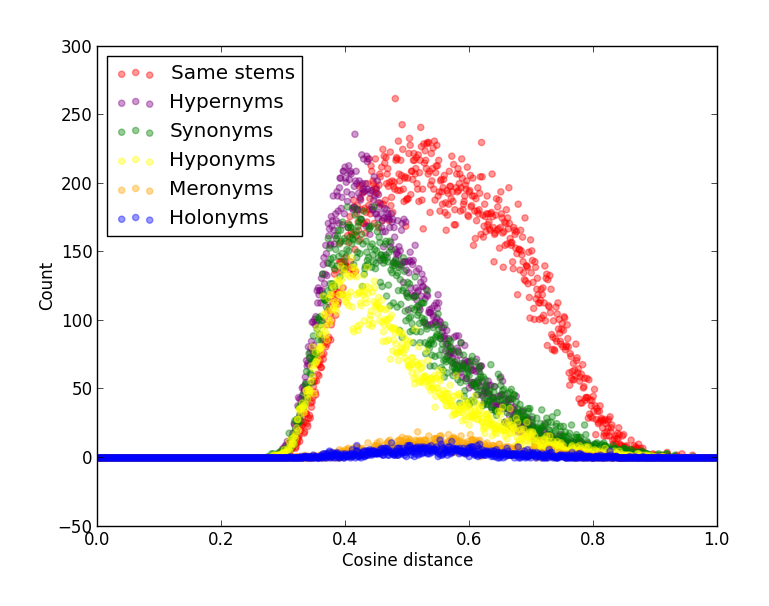
\includegraphics[scale=.5]{increment_lines.png}
  \captionsetup{justification=centering, margin=4cm }
  \caption{Relations are not distributed equivalently or uniformly across cosine distances. Cosine distances range from 0 to 1.}
  \label{fig:increment_lines.png}
\end{figure}

\subsection{Adjusted counts} \label{adjusted_counts}

We sampled 10,000 words in WordNet and found that any given word in WordNet has, on average, more hyponyms and synonyms than meronyms and holonyms. This follows partially from the structure of WordNet. Because WordNet is organized hierarchically as a tree \cite{clips}, any time a node branches, it creates n children. Each of the n children represents n hyponyms (the child nodes). But each node has exactly one parent. Thus, so long as the tree branches, the number of hyponyms for a given non-terminal node will outnumber its holonyms. We cannot account for the relative differences in meronyms, synonyms and holonyms from the structure of WordNet alone. 

\begin{figure}[!htbp]
\centering
\Tree [.carnivore [.feline [.{big cat} lion tiger ] cat ] [.canine dog wolf fox ] ]
\captionsetup{justification=centering, margin=4cm }
\caption{The downward-branching structure of WordNet shows why words have more hyponyms than hypernyms.}
\label{fig:wordnet}
\end{figure}

\begin{figure}[!htbp]
\centering
\begin{tabular}{ l | r }
  \hline                       
  Relation & Average Words in Wordnet \\ \hline
  Hyponym & 19.7 \\
  Synonym & 5.0 \\
  Hypernyms & 4.8 \\
  Meronym & 3.5 \\
  Holonym & 1.7 \\
  Average & 6.94 \\
  \hline  
\end{tabular}
\end{figure}

If some relations have more associated words than others, Word2Vec has more opportunities for finding a hit. This experiment seeks to measure Word2Vec, not WordNet. Thus, we adjust the counts from section \ref{binary} to account for varying numbers of types of relations. 

To find an adjusted count, we average the averages for each relation to get an overall average. For each relation, we find the ratio of its the average to the overall average. Then we multiply each (unadjusted) count by the inverse of the ratio. We repeat this at all values of k. For instance, for any average word, there are roughly 1/3 fewer total holonym words than average. So we multiply the holonym count by the inverse of this ratio (roughly 3).

\begin{figure}[!htbp]
  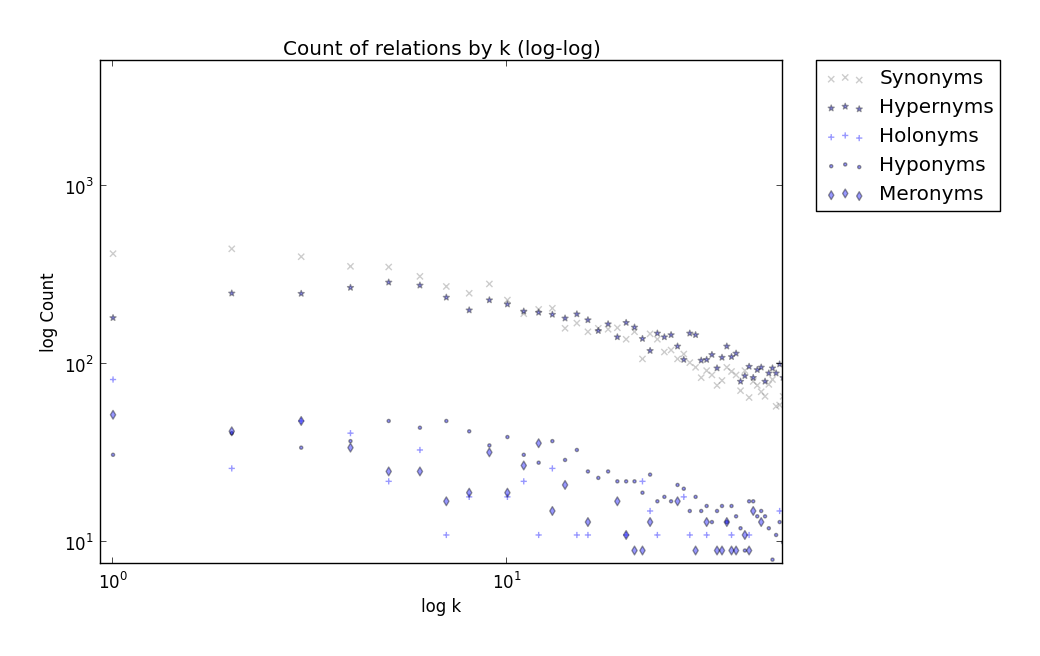
\includegraphics[scale=.5]{total_adjusted.png}
  \caption{For any given word in WordNet, the average number of words for each relation is dramatically different. Words have more hypernyms and holonyms than holonyms, for instance. We account for this with adjusted counts.}
  \label{fig:all_adjusted}
\end{figure}

Adjusted counts give a different perspective on Word2Vec. They show that, in general, Word2Vec returns more hypernyms than synonyms -- followed by far fewer hyponyms, holonyms and meronyms. 

\subsection{Cumulative counts} \label{binary}
Word2Vec returns words projected into a high-dimensional space. We might ask: what is the relationship of words that fall within a given semantic distance? We examine this question by calculating the cumulative counts for each relation at different semantic distances. 

In other words, if you were to draw something like a circle around a word in Word2Vec's the high-dimensional output 

\begin{figure}[!htbp]
  \centering
  \includegraphics[scale=.5]{total_by_semantic_cumulative.png}
  \captionsetup{justification=centering, margin=4cm }
  \caption{The total count of each relations beneath a given threshold levels off across all categories as the semantic distance increases.}
  \label{fig:all}
\end{figure}

\subsection{Probabilities}
Researchers who try to find particular kinds of relations using Word2Vec need to understand the baseline probability of the the relation at a particular semantic distance. An effective holonym detector, for instance, should beat the average probability of a holonym at a given semantic distance. 

\begin{table}[ht]
\centering
\small
\begin{tabulary}{\textwidth}{|R|R|R|R|R|R|R|R|}
\hline
Increment & Synonyms & Meronyms & Holonyms & Hypernyms & Hyponyms & Same stem & None \\  \hline
0.01 & 0.0 & 0.0 & 0.0 & 0.0 & 0.0 & 0.0 & 0.0 \\  \hline
0.029 & 0.0 & 0.0 & 0.0 & 0.0 & 0.0 & 0.0 & 0.0 \\  \hline
0.049 & 0.0 & 0.0 & 0.0 & 0.0 & 0.0 & 0.0 & 0.0 \\  \hline
0.069 & 0.0 & 0.0 & 0.0 & 0.0 & 0.0 & 0.0 & 0.0 \\  \hline
0.089 & 0.0 & 0.0 & 0.0 & 0.0 & 0.0 & 0.0 & 0.0 \\  \hline
0.109 & 0.0 & 0.0 & 0.0 & 0.0 & 0.0 & 0.0 & 0.0 \\  \hline
0.129 & 0.0 & 0.0 & 0.0 & 0.0 & 0.0 & 0.0 & 0.0 \\  \hline
0.149 & 0.0 & 0.0 & 0.0 & 0.0 & 0.0 & 0.0 & 0.0 \\  \hline
0.169 & 0.0 & 0.0 & 0.0 & 0.0 & 0.0 & 0.0 & 0.0 \\  \hline
0.189 & 0.0 & 0.0 & 0.0 & 0.0 & 0.0 & 0.0 & 0.0 \\  \hline
0.209 & 0.0 & 0.0 & 0.0 & 0.0 & 0.0 & 0.0 & 0.0 \\  \hline
0.229 & 0.0 & 0.0 & 0.0 & 0.0 & 0.0 & 0.0 & 0.0 \\  \hline
0.249 & 0.0 & 0.0 & 0.0 & 0.0 & 0.0 & 0.0 & 1.0 \\  \hline
0.269 & 0.004 & 0.0 & 0.0 & 0.0 & 0.0 & 0.0 & 0.996 \\  \hline
0.289 & 0.013 & 0.0 & 0.0 & 0.011 & 0.0 & 0.006 & 0.961 \\  \hline
0.309 & 0.014 & 0.0 & 0.0 & 0.012 & 0.0 & 0.008 & 0.95 \\  \hline
0.329 & 0.017 & 0.0 & 0.0 & 0.016 & 0.0 & 0.009 & 0.937 \\  \hline
0.349 & 0.017 & 0.0 & 0.0 & 0.015 & 0.0 & 0.011 & 0.935 \\  \hline
0.369 & 0.018 & 0.0 & 0.0 & 0.015 & 0.0 & 0.013 & 0.932 \\  \hline
0.389 & 0.019 & 0.0 & 0.0 & 0.015 & 0.0 & 0.016 & 0.926 \\  \hline
0.409 & 0.02 & 0.001 & 0.0 & 0.015 & 0.0 & 0.019 & 0.92 \\  \hline
0.429 & 0.02 & 0.001 & 0.0 & 0.015 & 0.0 & 0.024 & 0.914 \\  \hline
0.449 & 0.022 & 0.001 & 0.001 & 0.016 & 0.0 & 0.028 & 0.905 \\  \hline
0.469 & 0.023 & 0.001 & 0.001 & 0.015 & 0.0 & 0.033 & 0.9 \\  \hline
0.489 & 0.022 & 0.002 & 0.001 & 0.015 & 0.0 & 0.037 & 0.897 \\  \hline
0.51 & 0.021 & 0.002 & 0.001 & 0.014 & 0.0 & 0.042 & 0.894 \\  \hline
0.53 & 0.021 & 0.002 & 0.001 & 0.013 & 0.0 & 0.047 & 0.89 \\  \hline
0.55 & 0.02 & 0.003 & 0.001 & 0.012 & 0.0 & 0.048 & 0.892 \\  \hline
0.57 & 0.02 & 0.003 & 0.002 & 0.011 & 0.0 & 0.052 & 0.891 \\  \hline
0.59 & 0.019 & 0.003 & 0.001 & 0.011 & 0.0 & 0.06 & 0.883 \\  \hline
0.61 & 0.02 & 0.003 & 0.002 & 0.012 & 0.0 & 0.065 & 0.876 \\  \hline
0.63 & 0.02 & 0.003 & 0.001 & 0.011 & 0.0 & 0.076 & 0.869 \\  \hline
0.65 & 0.021 & 0.003 & 0.001 & 0.012 & 0.0 & 0.086 & 0.856 \\  \hline
0.67 & 0.022 & 0.003 & 0.002 & 0.013 & 0.0 & 0.097 & 0.843 \\  \hline
0.69 & 0.021 & 0.003 & 0.001 & 0.011 & 0.0 & 0.101 & 0.846 \\  \hline
0.71 & 0.019 & 0.003 & 0.002 & 0.01 & 0.0 & 0.106 & 0.847 \\  \hline
0.73 & 0.019 & 0.003 & 0.002 & 0.011 & 0.0 & 0.11 & 0.843 \\  \hline
0.75 & 0.021 & 0.002 & 0.001 & 0.009 & 0.0 & 0.121 & 0.831 \\  \hline
0.77 & 0.024 & 0.003 & 0.002 & 0.01 & 0.0 & 0.125 & 0.821 \\  \hline
0.79 & 0.025 & 0.002 & 0.002 & 0.011 & 0.0 & 0.126 & 0.818 \\  \hline
0.81 & 0.03 & 0.003 & 0.002 & 0.012 & 0.0 & 0.127 & 0.812 \\  \hline
0.83 & 0.034 & 0.005 & 0.005 & 0.015 & 0.0 & 0.111 & 0.811 \\  \hline
0.85 & 0.039 & 0.001 & 0.001 & 0.013 & 0.0 & 0.085 & 0.84 \\  \hline
0.87 & 0.029 & 0.001 & 0.001 & 0.011 & 0.0 & 0.059 & 0.888 \\  \hline
0.89 & 0.02 & 0.0 & 0.0 & 0.007 & 0.0 & 0.016 & 0.947 \\  \hline
0.91 & 0.034 & 0.004 & 0.002 & 0.009 & 0.0 & 0.015 & 0.928 \\  \hline
0.93 & 0.022 & 0.0 & 0.0 & 0.0 & 0.0 & 0.036 & 0.934 \\  \hline
0.95 & 0.0 & 0.0 & 0.0 & 0.0 & 0.0 & 0.031 & 0.969 \\  \hline
0.97 & 0.027 & 0.0 & 0.0 & 0.0 & 0.0 & 0.0 & 0.973 \\  \hline
0.99 & 0.0 & 0.0 & 0.0 & 0.0 & 0.0 & 0.0 & 1.0 \\  \hline
\end{tabulary}
\captionsetup{justification=centering}
\caption{This table demonstrates the empirical probabilities of finding a particular semantic relation at a particular cosine distance. Researchers may use such a table to establish an empirical baseline when seeking particular semantic relations.}
\label{tab:loglog_prob}
\end{table}


Our experiment has determined such probabilities at different cosine values. 

We present such probabilities in table  \ref{tab:loglog_prob}. We exclude meronyms and holonyms from this analysis because, as k increases past approximately 10, their probability becomes very very close to zero, as shown in figure \ref{fig:all}.


\subsection{Jaccard index} \label{Jaccard}
In our experiment, we use a binary measure of relatedness: if relevant synsets overlap, we consider the words related. Our experiment would determine that \textit{introduction} and \textit{initiation} are synonyms because their synsets overlap with the synset 'initiation.n.01'. This opens a potential complicating problem: the simple binary determination does not take into account that the word ``introduction" has seven associated synsets but the word ``initiation" has only 4 synsets -- and that these two sets overlap on a single synset. To account for the relative degree of overlap, we also take the Jaccard index of the overlapping sets to gain a better sense of the degree to which semantically related words are related. Our findings are shown in figure \ref{fig:jacard}.

\begin{figure}[!ht]
\centering
\centerline{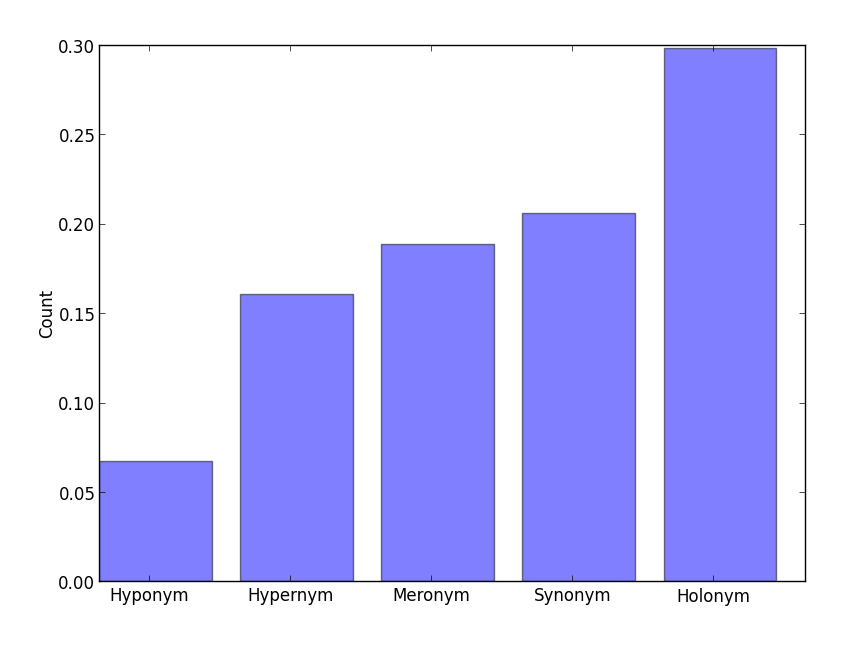
\includegraphics[scale=.5]{jacard.png}}
  \captionsetup{justification=centering, margin=4cm }
  \caption{Jaccard indexes vary depending on type of relation -- but the variation is closely correlated to the different sizes of synsets in WordNet}
  \label{fig:jacard}
\end{figure}

At first glance, figure \ref{fig:jacard} seems to show that Jaccard indexes vary. However, in section \ref{adjusted_counts} we sample 10,000 words from the Reuters corpus and find the average number of synonyms, hypoynms, hypernyms, holonyms and meronyms associated with each word (excluding cases where zero relations are found). Looking over both results, we see that Jaccard indexes for a given type of relation are strongly linked with the average synset sizes for each type of relation in WordNet.

In other words, the Jaccard index for holonyms is the highest among the relations -- but the holonymm set has the lowest average size in WordNet. Simiarly, the Jacard index for hypernyms is the lowest -- but hypernyms have the most associated words in WordNet. The union of two sets forms the denominator in the calculation of the Jaccard index. Thus, if there are higher numbers of one type of relation we would expect its Jaccard index to be lower (because the denominator would be larger). 

Differences in Jaccard indexes seem largely attributable to differences in synset sizes in WordNet (or perhaps in English), not to differences in the semantic relations uncovered by Word2Vec. 

\section{Future Work} \label{Future Work}

Comparing WordNet and Word2Vec is a limited topic and it has been thoroughly covered here. Most future work on Word2Vec will involve building tools and algorithms using word vectors. This study provides a clear baseline for such efforts. We hope that others use it to benchmark tools. 

That said a few matters of comparison have been left uncovered. 

In figure \ref{fig:all} we show that as k increases, Word2Vec eventually stops finding meronyms and holonyms (with any regularity). But it continues to find synonyms, hypernyms and hyponyms as k extends past 200. At what value of k does Word2Vec stop finding relations? This has not been answered in this study.

Additionally, this study uses one measure of semantic distance, the cosine distance -- which is explained in section \ref{method}.However, Word2Vec projects word vectors into semantic space. Thus, the system allows for any number of different measures of geometric distance, like Euclidean distance or Manhattan distance. Such geometric distances might yield different results. This might need to be investigated, depending on the particular needs at hand.

Word2Vec tracks the part of speech associated with a synset. We do not keep track of or use this information in this experiment. However, a follow up experiment that examines how differences in part of speech impact results could yield insights into both Word2Vec and distributional semantics. After all, the fundamental hypothesis underlying distributional semantics is that words that appear together in language -- like \textit{piano} and \textit{keys} -- have related meanings. This might be true for nouns or verbs but might not be as true for adjectives or adverbs. The word \textit{good} is used to describe many different things. There is no particular reason to think that it is semantically closer to the word that it modifies. Note that in Word2Vec, words are not assigned a part of speech, so in some cases the contextual part of speech will be ambiguous.

Finally, this study only considered the text of news articles. It would be interesting to compare Word2Vec's performance on different sorts of text. Do news articles tend to favor words at higher levels of generality (hypernyms) over words at lower level of generality (hyponyms)? If different kinds of raw text contain kinds of language, Word2Vec might find different sorts of most-similar words. Thus experimenters might find different results.

\section{Conclusion}

There are many ways that words may be semantically related. We show that certain semantic relations are more probable than other semantic relations in output from Word2Vec. More precisely, we show that for some word \textit{w}, we find the probability that a neighbor at a given cosine distance is a synonym, a hypernym, a holonym or a meronym. 

\clearpage

\bibliographystyle{unsrt}%Used BibTeX style is unsrt
\bibliography{sample}

\clearpage

\section{Vita}
\noindent\fbox{%
    \parbox{\textwidth}{%
Abe Handler currently works as a software developer and data journalist for \textit{The Lens}, an online, non-profit investigative newsroom. He entered the Masters program in Computer Science at the University Of New Orleans in 2012. He is interested in information retrieval, natural language processing, machine learning and data science -- especially as it pertains to law, politics, social science and journalism. Abe holds a B.A. in philosophy from Columbia University, where he reported for the student newspaper \textit{The Columbia Daily Spectator} -- graduating with honors in 2007.
    }%
}


\end{document}
